\documentclass[10pt,a4paper]{amsart}
\usepackage[margin=19mm]{geometry}
\usepackage{amsmath,amssymb,mathtools}
\usepackage[scr=rsfs,cal=euler]{mathalfa}
\usepackage{xfrac}
\usepackage[unicode,hidelinks,bookmarks=false]{hyperref}
\newcommand{\ie}{i.e.\ }
\newcommand{\cf}{cf.\ }
\newcommand{\resp}{respectively\ }
\newcommand{\Subsection}{\subsection}
\providecommand{\nobreakdash}{\nobreak\hbox{-}}
\setlength{\emergencystretch}{2em}
\multlinegap0pt
\usepackage{tikz}
\usepackage{float}
\usepackage{amssymb}
\usepackage{mathtools}
\usepackage{cancel}
\usepackage[shortlabels]{enumitem}
\newtheorem{lemma}{Lemma}
\usepackage{cleveref}
\crefname{lemma}{Lemma}{Lemmas}
\title{On the dimension drop for harmonic measure on uniformly non-flat Ahlfors-David regular boundaries.}
\author{Aritro Pathak}
\date{Source: arXiv:2601.16167v3 (CC BY 4.0)}
\begin{document}
\maketitle

\noindent\emph{Source and licence.} On the dimension drop for harmonic measure on uniformly non-flat Ahlfors-David regular boundaries.. Version arXiv:2601.16167v3 (CC BY 4.0), distributed by arXiv under the Creative Commons Attribution 4.0 International licence, http://creativecommons.org/licenses/by/4.0/, as recorded in the arXiv licence metadata for this exact version and shown on the abstract page https://arxiv.org/abs/2601.16167v3. Full licence notice: \texttt{licenses/arxiv-2601.16167-CC-BY-4.0.txt}.\par\smallskip

\noindent\textit{Editorial scope.} Counted unit: the article's lemma eq10 (source0.tex lines 609--614). The article's complete original proof of it is delivered with it (source0.tex lines 616--708, one \texttt{proof} environment of 93 lines). No mathematics is written, repaired or re-derived: the statement and the proof are the article's own lines, in the article's own notation, and no retained line is substituted or re-flowed.  No further source-local context is needed: every cross-reference of every retained line resolves inside the two delivered spans.  Nothing was omitted from any retained span, so the package carries no omission record.  No retained line contains a citation, so the wrapper carries no bibliography and no bibliography entry.  The retained lines contain the article's own diagram code, which the wrapper typesets with the standard tikz packages; no image file is delivered and the package declares no asset dependency.  Editorial formatting only, in addition: an AMS \texttt{amsart} preamble that restates the article's own declarations and macros used by the retained lines, namely the environments \texttt{lemma} on separate counters, together with the standard packages those lines need.  The retained environments print in this document as Lemma 1 in order of appearance, whereas the article prints the same items with the numbering of its own full document.  The complete native source of the article as distributed in the arXiv e-print for this exact version is bundled unchanged as \texttt{sources/193219/source0.tex}.
      \begin{lemma}
          Consider the cube $C(q_1,t_1)$. Then there exists a $1 \leq \kappa\leq \frac{1}{2}$ so that we have the following decomposition of the ball $C(q_1,t_1):=\cup_{m\geq 0}C(q_1,\kappa^m t_1)\setminus C(q_1,\kappa^{m+1}t_1) :=A(q_1,m)$, so that, 
        \begin{align}\label{eq10}
    \frac{1}{2}  C_{1}^{-1} \kappa^{ms}t_{1}^{s}\leq \sigma(A_m (q_1))\leq C_1 \kappa^{ms} t_{1}^s
\end{align}
      \end{lemma}

      \begin{proof}Consider the following decomposition of this cube $B(q_1,t_1)$: depending on the Ahlfors David regularity constant $C_1$. We consider the value $0<\kappa<1$ so that,
      \begin{align}\label{ample}
            C_{1}^{-1} t_{1}^s -C_{1}(\kappa t)^s \geq \frac{1}{2}  C_{1}^{-1} t_{1}^{s}\Leftrightarrow \kappa \leq C_{1}^{-2/s}.
      \end{align}

     Consider the unique positive integer $N$ so that, $\frac{1}{N+1}<C_{1}^{-2/s}\leq \frac{1}{N}$. Thus, $N=\lceil C_{1}^{2/s} \rceil$. We choose a value of 
     \begin{align}\label{kappa}
    \kappa=\frac{1}{4N+2}= \frac{1}{4\lceil C_{1}^{2/s} \rceil +2}.
    \end{align}
     In particular, we have $\kappa\leq \frac{1}{2}$.
     
     \begin{figure}
     \centering

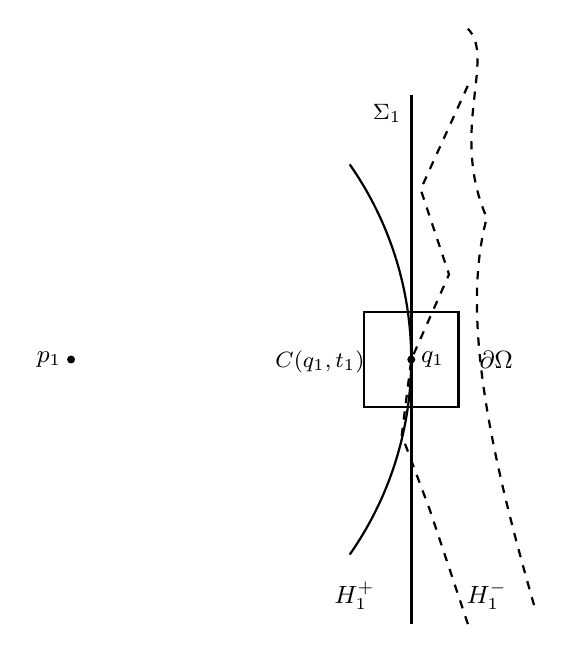
\begin{tikzpicture}[
    scale=1.2,
    every node/.style={font=\small}
]

\def\r{3.6}
\def\tone{1}

\coordinate (p1) at (0,0);
\coordinate (q1) at (\r,0);

% Arc (leftmost boundary constraint)
\draw[thick]
  ({\r*cos(-35)}, {\r*sin(-35)})
  arc[start angle=-35, end angle=35, radius=\r];

% Hyperplane Sigma_1 (bold)
\draw[very thick] (\r,-2.8) -- (\r,2.8);
\node[above left, font=\footnotesize] at (\r,2.4) {$\Sigma_1$};

% Irregular dashed boundary strands
% (some portions lie left of Sigma_1, all right of the arc)

% Main strand through q1
\draw[dashed, thick]
  (\r+0.6,-2.8)
    -- (\r+0.2,-1.6)
    -- (\r-0.1,-0.8)
    -- (q1)
    -- (\r+0.4,0.9)
    -- (\r+0.1,1.8)
    -- (\r+0.6,2.9);

% Secondary strand
\draw[dashed, thick]
  (\r+1.3,-2.6)
    .. controls (\r+0.9,-1.2) and (\r+0.5,0.4) ..
  (\r+0.8,1.5)
    .. controls (\r+0.4,2.4) and (\r+0.9,3.2) ..
  (\r+0.6,3.5);

% Points
\fill (p1) circle (1.2pt);
\node[left] at (p1) {$p_1$};

\fill (q1) circle (1.2pt);
\node[right] at (q1) {$q_1$};

% Half-planes
\node at (\r-0.6,-2.5) {$H_1^{+}$};
\node at (\r+0.8,-2.5) {$H_1^{-}$};
\node at (\r+0.9,0) {$\partial\Omega$};

% Cube at q1
\draw[thick]
  (\r-0.5,-0.5) rectangle (\r+0.5,0.5);

\node[above right, font=\footnotesize]
  at (\r-1.54,-0.25) {$C(q_1,t_1)$};

\end{tikzpicture}

\caption{The corkscrew point $p_1$ and a point $q_1\in\partial\Omega$ nearest to $p_1$ is shown in the figure. The hyperplane $\Sigma_1$ passes through $q_1$ and is perpendicular to the line joining $p_1,q_1$, and the cube $C(q_1,t_1)$ is also shown. The left and right half planes in the figure are respectively $H^{+}_1, H^{-}_1$. The arc shows a portion of the sphere $S(p_1, r_1)$. The dashed lines depict the boundary $\partial\Omega$, which lies in the complement of the ball $B(p_1,r_1)$.}
\end{figure}

This ensures that for the annular region $\sigma(C(q_1,t_1)\setminus C(q_1,\kappa t_1))\geq \frac{1}{2}  C_{1}^{-1} t_{1}^{s} $. Further, we trivially have an upper bound of $\sigma(C(q_1,t_1)\setminus C(q_1,\kappa t_1))\leq C_1 t_{1}^s$, for the amount of surface measure within this region. Thus we have, 
\begin{align}\label{eq6}
    \frac{1}{2}  C_{1}^{-1} t_{1}^{s}\leq \sigma(C(q_1,t_1)\setminus C(q_1,\kappa t_1))\leq C_1 t_{1}^s
\end{align}

Successively, we consider for each integer $m\geq 0$, the annular regions, 
\begin{align}
    A_m (q_1):= C(q_1,\kappa ^m t_1)\setminus C(q_1,\kappa^{m+1} t_1).
\end{align}

By the same argument as that for \cref{eq6}, we also get that,
\begin{align}
    \frac{1}{2}  C_{1}^{-1} \kappa^{ms}t_{1}^{s}\leq \sigma(A_m (q_1))\leq C_1 \kappa^{ms} t_{1}^s
\end{align}\end{proof}

\end{document}
